\section{并发执行}

数据库系统允许多个事务并发运行。

并发执行的优点如下:
\begin{itemize}
    \item 提高处理器和磁盘利用率,从而提高事务吞吐量:一个事务使用CPU时,另一个事务可以进行磁盘读写操作。
    \item 减少事务的平均响应时间:短事务无需等待长事务。
\end{itemize}

问题:尽管每个单独的事务都是正确的,但并发可能会破坏数据的一致性。(如并发售票问题)

并发控制方案——实现隔离的机制,即控制并发事务之间的交互,以防止它们破坏数据库的一致性。——这是数据库管理系统的重要工作

这里我们研究并发执行的正确性、可串行化、可恢复性等概念。

\noindent\textbf{调度}——指示并发事务的指令执行时间顺序的序列
\begin{itemize}
    \item 一组事务的调度必须包含这些事务的所有指令
    \item 必须保留指令在每个单独事务中出现的顺序。
\end{itemize}

\begin{figure}[H]
    \centering
    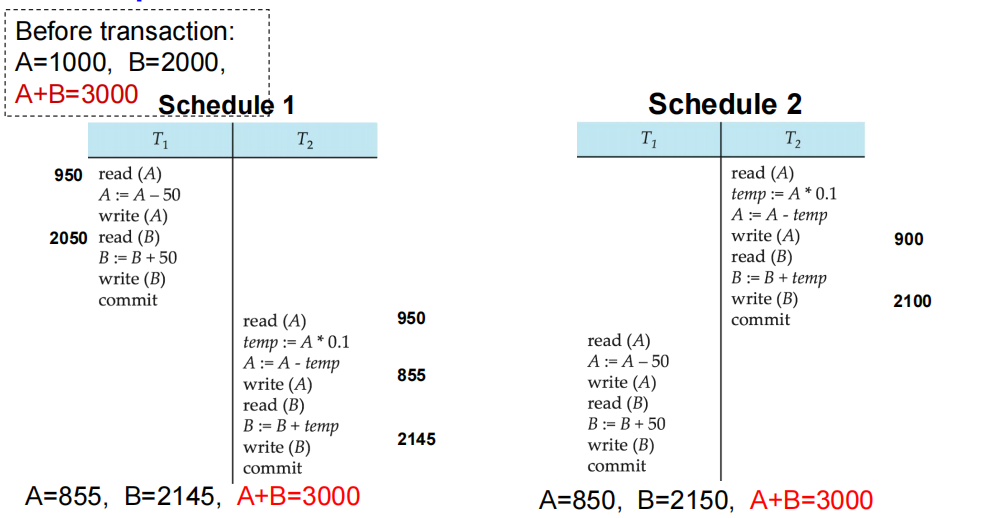
\includegraphics[width=0.8\linewidth]{image4.png}
    \caption{}
    \label{}
\end{figure}

调度1和调度2均为串行调度。

N个并行事务有n!种可选的串行调度。串行调度必定保持一致性,但是效率低下。